\documentclass[doktyp=semarbeit, sprache=german]{TUBAFarbeiten}
\usepackage[utf8]{inputenc}
\usepackage[T1]{fontenc}
\usepackage{graphicx} 
\usepackage{amsmath}
\usepackage{subcaption}
\usepackage{booktabs}
\usepackage{url}
\usepackage{listings}
\lstset{
  language=bash,
  basicstyle=\ttfamily
}
\lstnewenvironment{CPP}
  {\lstset{language=C++,basicstyle=\ttfamily\small,frame=none}}
  {}
\captionsetup{compatibility=false}
\bibliographystyle{unsrt}
\TUBAFFakultaet{Fakultät für Mathematik und Informatik}
\TUBAFInstitut{Institut für Informatik}
\TUBAFLehrstuhl{Lehrstuhl für Betriebssysteme und Kommunikationstechnologien}
\TUBAFTitel{Aufbau eines Prototyps für verteilte CUDA Programmierung}
\TUBAFUntertitel{Development of a prototype for distributed CUDA programming}
\TUBAFKorrektor{Dr. rer. nat. Martin Reinhardt}
\TUBAFBetreuer{Prof. Dr. Konrad Froitzheim}
\TUBAFAutor[S. Dressel]{Samuel Dressel}
\TUBAFStudiengang{Angewandte Informatik}
\TUBAFVertiefung{Parallelrechner}
\TUBAFMatrikel{59963}
\TUBAFDatum{\today}
\begin{document}
\maketitle
\tableofcontents
\TUBAFErklaerungsseite
\newpage
\section{Einleitung}
\section{Grundlagen}
\subsection{Message-Passing-Interface (MPI)}
Das Message-Passing-Interface, kurz MPI, ist eine standartisierte Schnittstelle für die Kommunikation auf verteilten Systemen. Es wird häufig wissenschaftlichen und ingenieurstechnischen Domänen verwendet, um größere Problemstellungen effizienter zu bearbeiten und zu lösen \cite{MPIBook}. MPI ist speziell für die Verwendung auf verteilten Systemen mit ebenso verteiltem Speicher konstruiert. Dabei kann jeder Prozessor, der Teil der Bearbeitung eines Workloads ist, nur auf seinen lokalen Speicher zugreifen. Es können jedoch durch Messages Daten von einem lokalen Speicher in den anderen übertragen werden.
\\MPI ist als Bibliothek implementiert, nicht als Programmiersprache. Dabei existieren Implementierungen für zahlreiche Programmiersprache wie C, C++, Python oder Fortran \cite{ScriptPC}.
\\Die grundlegendste Art der Kommunikation findet zwischen zwei Prozessen statt. Dabei übermittelt ein Sendeprozess Informationen an einen Empfangsprozess.
\begin{figure}
	\centering
	\captionsetup{justification=centering} 
	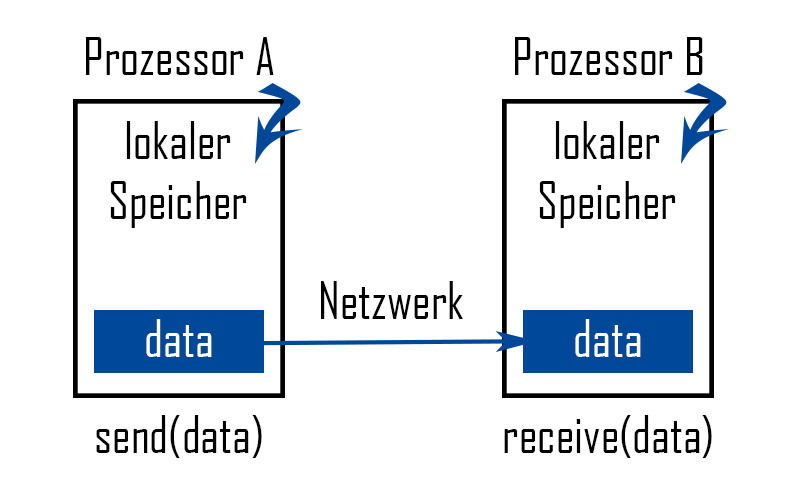
\includegraphics[width=1.0\textwidth]{images/MPIModell.jpg}
	\caption{Grundlegendes Konzept von MPI: Ein Sendeprozess sendet Daten an einen Empfangsprozess über ein Netzwerk. Jeder Prozess kann nur unmittelbar auf seinen zugehörigen lokalen Speicher zugreifen.}
	\label{img:mpimodell}
\end{figure}
Prozesse lassen sich außerdem in Gruppen zusammenfassen, wobei jeder Prozess eine eindeutige Nummer (Rang bzw. Rank) zugeorndet wird. Der Zugriff auf diese Gruppe wird über einen Kommunikator gesteuert. Innerhalb dieser Gruppe können mithilfe einer Boradcast-Operation von einem Masterprozess allen anderen Prozessen Nachrichten gesendet werden. Diese zurückgegebenen Daten werden mithilfe einer Gather-Funktion wieder eingesammelt.
\\Dieses Konzept wird auch für den im Rahmen dieser Arbeit erstellten Minicluster genutzt: Der Workload wird von dem Masterknoten definiert und dann über das Message-Passing-Interface and die Work-Nodes (Arbeitsknoten) gesendet. Dies erlaubt dann letztendlich die Verteilung der Workload innerhalb des Clusters.
\subsection{CUDA}
Im Vergleich zu einer CPU besteht eine Grafikkarte aus einer großen Anzahl parallel nutzbarer Kerne, die eine Vielzahl von Berechnungen parallel ausführen können. Beispielsweise besitzt eine \textit{NVIDIA RTX 2080} 2944 CUDA-Kerne, während die meisten CPUs 8 bis 16 Kerne besitzen \cite{RTXCores}. 
Natürlich sind die Kerne ein GPU in ihrer Struktur und Instruktionskomplexität wesentlich einfacher, da sie dafür ausgelegt sind, Aufgaben als Gruppe zu bearbeiten.
Eine CPU ist auf generelle Programmanforderungen ausgelegt und muss eine Vielzahl von Befehlen und Datentypen unterstützen. Eine GPU ist hingegen auf Grafikberechnungen spezialisiert und in ihrer grundlegenden Funktion für Pixelberechnungen konzipiert worden.
\\Aufgrund dieser Struktur lassen sich GPUs aber nicht nur für Grafikberechnungen nutzen, sondern auch bei der Berechnung von wissenschaftlichen Problemen.
Um diese Architektur nutzen und steuern zu können, wurde die Programmierschnittstelle CUDA (\textit{Compute Unified Device Architecture}) entwickelt. CUDA wurde dabei von NVIDIA entwickelt und erlaubt die Beschleunigung von Programmen, indem neben der CPU bestimmte Programmteile von einer oder mehreren GPUs parallelisiert bearbeitet werden.
\\CUDA besitzt Bindings für viele wissenschaftlich genutzte Programmiersprachen wie C/C++, Fortran oder Python und ist mit allen herkömmlichen Betriebssystemen kompatibel \cite{CUDADefinition}.
\subsection{CUDA und MPI}
Sowohl CUDA als auch MPI dienen in ihrer grundlegenden Funktion zur Bereitstellung einer Schnittstelle von parallelen bzw. verteilten Berechnungen. MPI erlaubt es wie schon oben erwähnt, bestimmte Aufgaben innerhalb eines verteilten Systems zu koordinieren und aufzuteilen. Grundsätzlich wird dabei nur die Rechenleistung der einzelnen Prozessoren genutzt \cite{CUDAAwareMPI}.
Für eine weitere Optimierung durch Verwendung von verschiedenen GPUs in einem verteilten System ist zusätzlich CUDA als GPU-Schnittstelle notwendig.
Dabei ergibt sich jedoch folgendes Problem: Standartmäßig werden bei der Verwendung von MPI nur Zeiger auf den Hauptspeicher des Hosts weitergeleitet. Jedoch müssen bei der Kombination von MPI und CUDA meist GPU-Buffer gesendet werden. Hierzu müssen diese Buffer zunächst in den Hauptspeicher kopiert werden, um dann gesendet werden zu können:
\begin{CPP}
//MPI rank 0
cudaMemcpy(s_buf_h,s_buf_d,size,cudaMemcpyDeviceToHost);
MPI_Send(s_buf_h,size,MPI_CHAR,1,100,MPI_COMM_WORLD);

//MPI rank 1
MPI_Recv(r_buf_h,size,MPI_CHAR,0,100,MPI_COMM_WORLD, &status);
cudaMemcpy(r_buf_d,r_buf_h,size,cudaMemcpyHostToDevice);
\end{CPP}
Diese Tatsache führt zu erheblichen Zeitverlusten und kann eine Optimierung von Berechnung mit CUDA und MPI einschränken. Daher wurde eine Vielzahl von MPI-Implementation wie \textit{MVAPICH2} oder \textit{OpenMPI} um eine spezielle CUDA-Unterstützung erweitert. Diese Unterstützung trägt den Namen \textit{CUDA-aware MPI}. Mit CUDA-aware MPI können GPU-Buffer direkt an MPI weitergegeben werden:
\begin{CPP}
//MPI rank 0
MPI_Send(s_buf_d,size,MPI_CHAR,1,100,MPI_COMM_WORLD);

//MPI rank n-1
MPI_Recv(r_buf_d,size,MPI_CHAR,0,100,MPI_COMM_WORLD, &status);
\end{CPP}
Dabei muss eine CUDA-aware MPI-Implementation unterscheiden, ob der jeweilige Buffer auf dem Hostspeicher oder dem Speicher der GPU liegt. Seit der CUDA-Version 4.0 wurde das CUDA-Feature UVA (\textit{Unified Virtual Addressing}) eingeführt, welches den Hauptspeicher und den Gerätespeicher kombiniert und einem virtuellen Adressraum zusammenfasst.
\begin{figure}
	\centering
	\captionsetup{justification=centering} 
	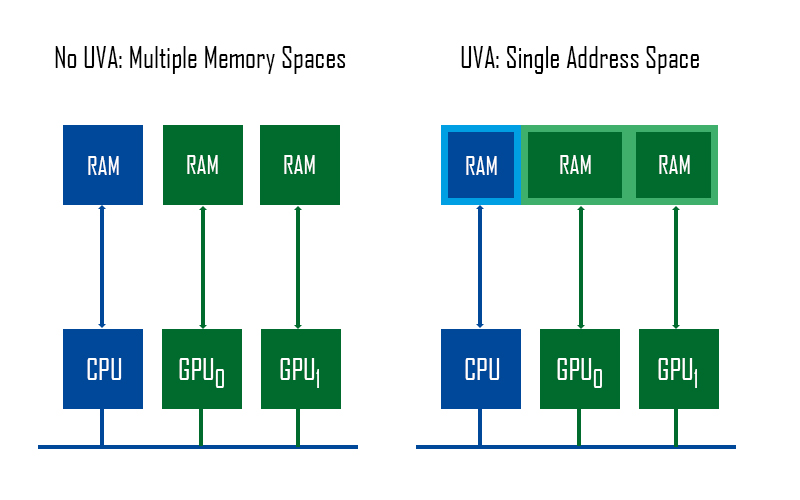
\includegraphics[width=1.0\textwidth]{images/CUDAUVA.jpg}
	\caption{Links ist das Speicherhandling ohne UVA abgebildet, rechts das Speicherhandling mit UVA. Bei der Nutzung von Unified Virtual Addressing werden die Speicherräume aller System- und Gerätespeicher in einem virtuellen Adressraum zusammengefasst.}
	\label{img:cudauval}
\end{figure}
Ein weiteres Feature von CUDA, eingeführt mit der Version 5.0, ist die \textit{GPUDirect}-Funktionalität. Dies erlaubt mithilfe des \textit{Remote Direct Memory Access} (RDMA) das direkte Senden von Grafikspeicher an den Netzwerkadapter ohne Routing über den jeweiligen Hauptspeicher. 
%Bild
Diese Funktionen bilden die Grundlage für eine gelungene Optimierung von verteilten Berechnungen auf verteilten Systemen durch Nutzung von CUDA-aware MPI.
\section{Technischer Aufbau und Konfiguration}
Für den Aufbau des Mini-Clusters werden zunächst folgende Dinge benötigt:
\begin{itemize}
	\item Nvidia Jetson Nano (3x)
	\item SD-Karte (3x)
	\item Ethernet-Kabel (4x)
	\item 4-Port Ethernet Switch
	\item Optional: 40mm Lüfter (3x, in diesem Fall wurde der Noctua NF-A4x20 verwendet)
\end{itemize}
Der technische Aufbau beginnt mit der physischen Verbindung der Nvidia Jetson Nanos. Dazu werden diese alle via Ethernet-Kabel mit einem Ethernet Switch verbunden, welcher wiederum durch LAN mit einem Router und dadurch mit dem Internet verbunden ist. An sich benötigt der Cluster keinen Internetzugang, für die Einrichtung ist dieser jedoch unersetzlich. Einer der Jetson Nanos fungiert als Head-Node (Masterknoten), die anderen zwei als Worker-Nodes.
\\Ist das physische Setup abgeschlossen, wird als nächstes auf jedem der Jetson Nanos das Jetson Nano Developer Kit SD Card Image installiert. Dies geschieht durch das Schreiben des Images auf die jeweilige SD-Karte und einem anschließenden Setup auf den Jetson Nanos \cite{SDImage}. Danach wird das System durch Aktualisierung der Pakete auf den neuesten Stand gebracht:
\begin{lstlisting}
sudo apt-get update
sudo apt-get upgrade
\end{lstlisting}
Es folgt die Installation des \texttt{nano}-Texteditors und des SSH-Paketes. Dabei ist SSH für den Remotezugriff auf die einzelnen Knoten notwendig; an Stelle des \texttt{nano}-Texteditors kann alternativ jeder andere Editor benutzt werden.
\begin{lstlisting}
sudo apt-get install nano
sudo apt-get install openssh-server
\end{lstlisting}
Zusätzlich ist auf dem Masterknoten der NFS-Kernel-Server zu installieren:
\begin{lstlisting}
sudo apt-get install nfs-kernel-server
\end{lstlisting}
Auf den Worker-Nodes wird dagegen das \texttt{nfs-common}-Paket installiert:
\begin{lstlisting}
sudo apt-get install nfs-common
\end{lstlisting}
NFS und die damit verbundenen Pakete sind notwendig, um später Dateien innerhalb des Clusters auszutauschen.
\\Um dieses Netzwerk einzurichten, muss zunächst jedem der drei Knoten eine statische IP zugewiesen werden. Dies erfolgt entweder über die Netzwerkeinstellungen oder über das Bearbeiten der Interface-Datei:
\begin{lstlisting}
cd /etc/network
sudo nano interfaces
\end{lstlisting}
Dafür werden der Datei folgende Zeilen hinzugefügt:
\begin{lstlisting}
auto eth0
iface eth0 inet static
address 192.168.178.10
gateway 192.168.178.1
netmask 255.255.255.0
\end{lstlisting}
Dabei ist die Adresse \texttt{192.168.178.10} die Adresse des Masterknotens, die Worker-Nodes erhalten dann dementsprechend die IP-Adressen \texttt{192.168.178.11} und \texttt{192.168.178.12}. Damit die Änderungen wirksam werden, müssen entweder die Jetson Nanos oder der Network-Service neugestartet werden.
\\Als nächstes erfolgt die Einrichtung von SSH innerhalb des Clusters. Dazu wird zuerst jedem Knoten ein Name zur besseren Identifikation zugewiesen. Hierfür wird die \texttt{hostname}-Datei bearbeitet:
\begin{lstlisting}
sudo nano /etc/hostname
\end{lstlisting}
Der Masterknoten erhält in diesem Fall den Namen \texttt{master}, die Worker-Nodes die Namen \texttt{slave1} und \texttt{slave2}. Als nächstes werden in der \texttt{hosts}-Datei die statischen IP-Adressen aller Knoten hinzugefügt. Dies geschieht wie der vorige Schritt auf allen Knoten:
\begin{lstlisting}
sudo nano /etc/hosts
\end{lstlisting}
Die \texttt{hosts}-Datei sollte dann so aussehen:
\begin{lstlisting}
192.168.178.10 master
192.168.178.11 slave1
192.168.178.12 slave2
\end{lstlisting}
Nach dem Einrichten der statischen IP-Adressen folgt nun das Setup von SSH. Dazu wird zunächst ein 2048 bit RSA Schlüsselpaar auf dem Masterknoten erstellt:
\begin{lstlisting}
ssh-keygen -t rsa -b 2048
\end{lstlisting}
Danach wird die SSH ID an alle Knoten inklusive des Masterknotens weitergeben:
\begin{lstlisting}
ssh-copy-id master
ssh-copy-id slave1
ssh-copy-id slave2
\end{lstlisting}
Eine Kommunikation zwischen den Knoten ohne ständige Passwort- bzw. Berechtigungsabfrage ist für die Funktionalität des Cluster von großer Bedeutung. Dies geschieht durch das Generieren der \texttt{known\_hosts}-Datei im \texttt{.ssh}-Ordner.  Dazu wird zunächst eine Datei mit den Namen aller Knoten im \texttt{.ssh}-Ordner angelegt:
\begin{lstlisting}
cd .ssh
sudo nano name_of_hosts
\end{lstlisting}
Die Datei enthält dann folgende Einträge:
\begin{lstlisting}
master
slave1
slave2
\end{lstlisting}
Damit der \texttt{ssh-keyscan} die Datei lesen kann, müssen anschließend die Zugriffsberechtigungen geändert werden:
\begin{lstlisting}
sudo chmod 666 ~/.ssh/name_of_hosts
\end{lstlisting}
Mit folgendem Befehl wird letztendlich die \texttt{known\_hosts}-Datei erzeugt:
\begin{lstlisting}
ssh-keyscan -t rsa -f ~/.ssh/name_of_hosts >~/.ssh/known_hosts
\end{lstlisting}
Als letztes muss diese Datei und die notwendigen Schlüssel noch an die anderen Knoten kopiert werden:
\begin{lstlisting}
cd .ssh
scp known_hosts id_rsa id_rsa.pub nvidia@master:.ssh
scp known_hosts id_rsa id_rsa.pub nvidia@slave1:.ssh
scp known_hosts id_rsa id_rsa.pub nvidia@slave2:.ssh
\end{lstlisting}
Der letzte Schritt der Konfiguration ist das Erstellen und Mounten eines gemeinsamen Arbeitsordners für alle Knoten. Hierfür das Network File System benutzt, dessen Pakete anfangs installiert wurden. Auf dem Masterknoten wird dabei als erstes dieser Arbeitsordner erstellt:
\begin{lstlisting}
sudo mkdir /cloud
\end{lstlisting}
Danach muss die \texttt{exports}-Datei auf dem Masterknoten editiert werden:
\begin{lstlisting}
sudo nano /etc/exports
\end{lstlisting}
Diese Datei enthält alle Informationen über das Exportieren des Arbeitsordners auf die einzelnen Knoten:
\begin{lstlisting}
/cloud slave1(rw,sync,no_root_squash,no_subtree_check)
/cloud slave2(rw,sync,no_root_squash,no_subtree_check)
\end{lstlisting}
Die zwei Worker-Nodes müssen nun diesen gemeinsamen Arbeitsordner mounten. Dazu wird auf jedem Worker-Node der \texttt{cloud}-Ordner erstellt und mithilfe des Editierens der \texttt{fstab}-Datei gemountet:
\begin{lstlisting}
sudo mkdir /cloud
sudo nano /etc/fstab

master:/cloud /cloud nfs rsize=8192,wsize=8192,timeo=14,intr
\end{lstlisting}
Der technische Aufbau und die Konfiguration des Clusters ist hiermit abgeschlossen.
\section{CUDA und MPI}

\section{Benchmarking und Test ausgewählter Algorithmen}
\section{Fazit}
\newpage
\addcontentsline{toc}{section}{\protect\numberline{}{Anhang}} 
\begin{appendix} 
\section{Aufbau des Clusters}
\begin{figure}
	\centering
	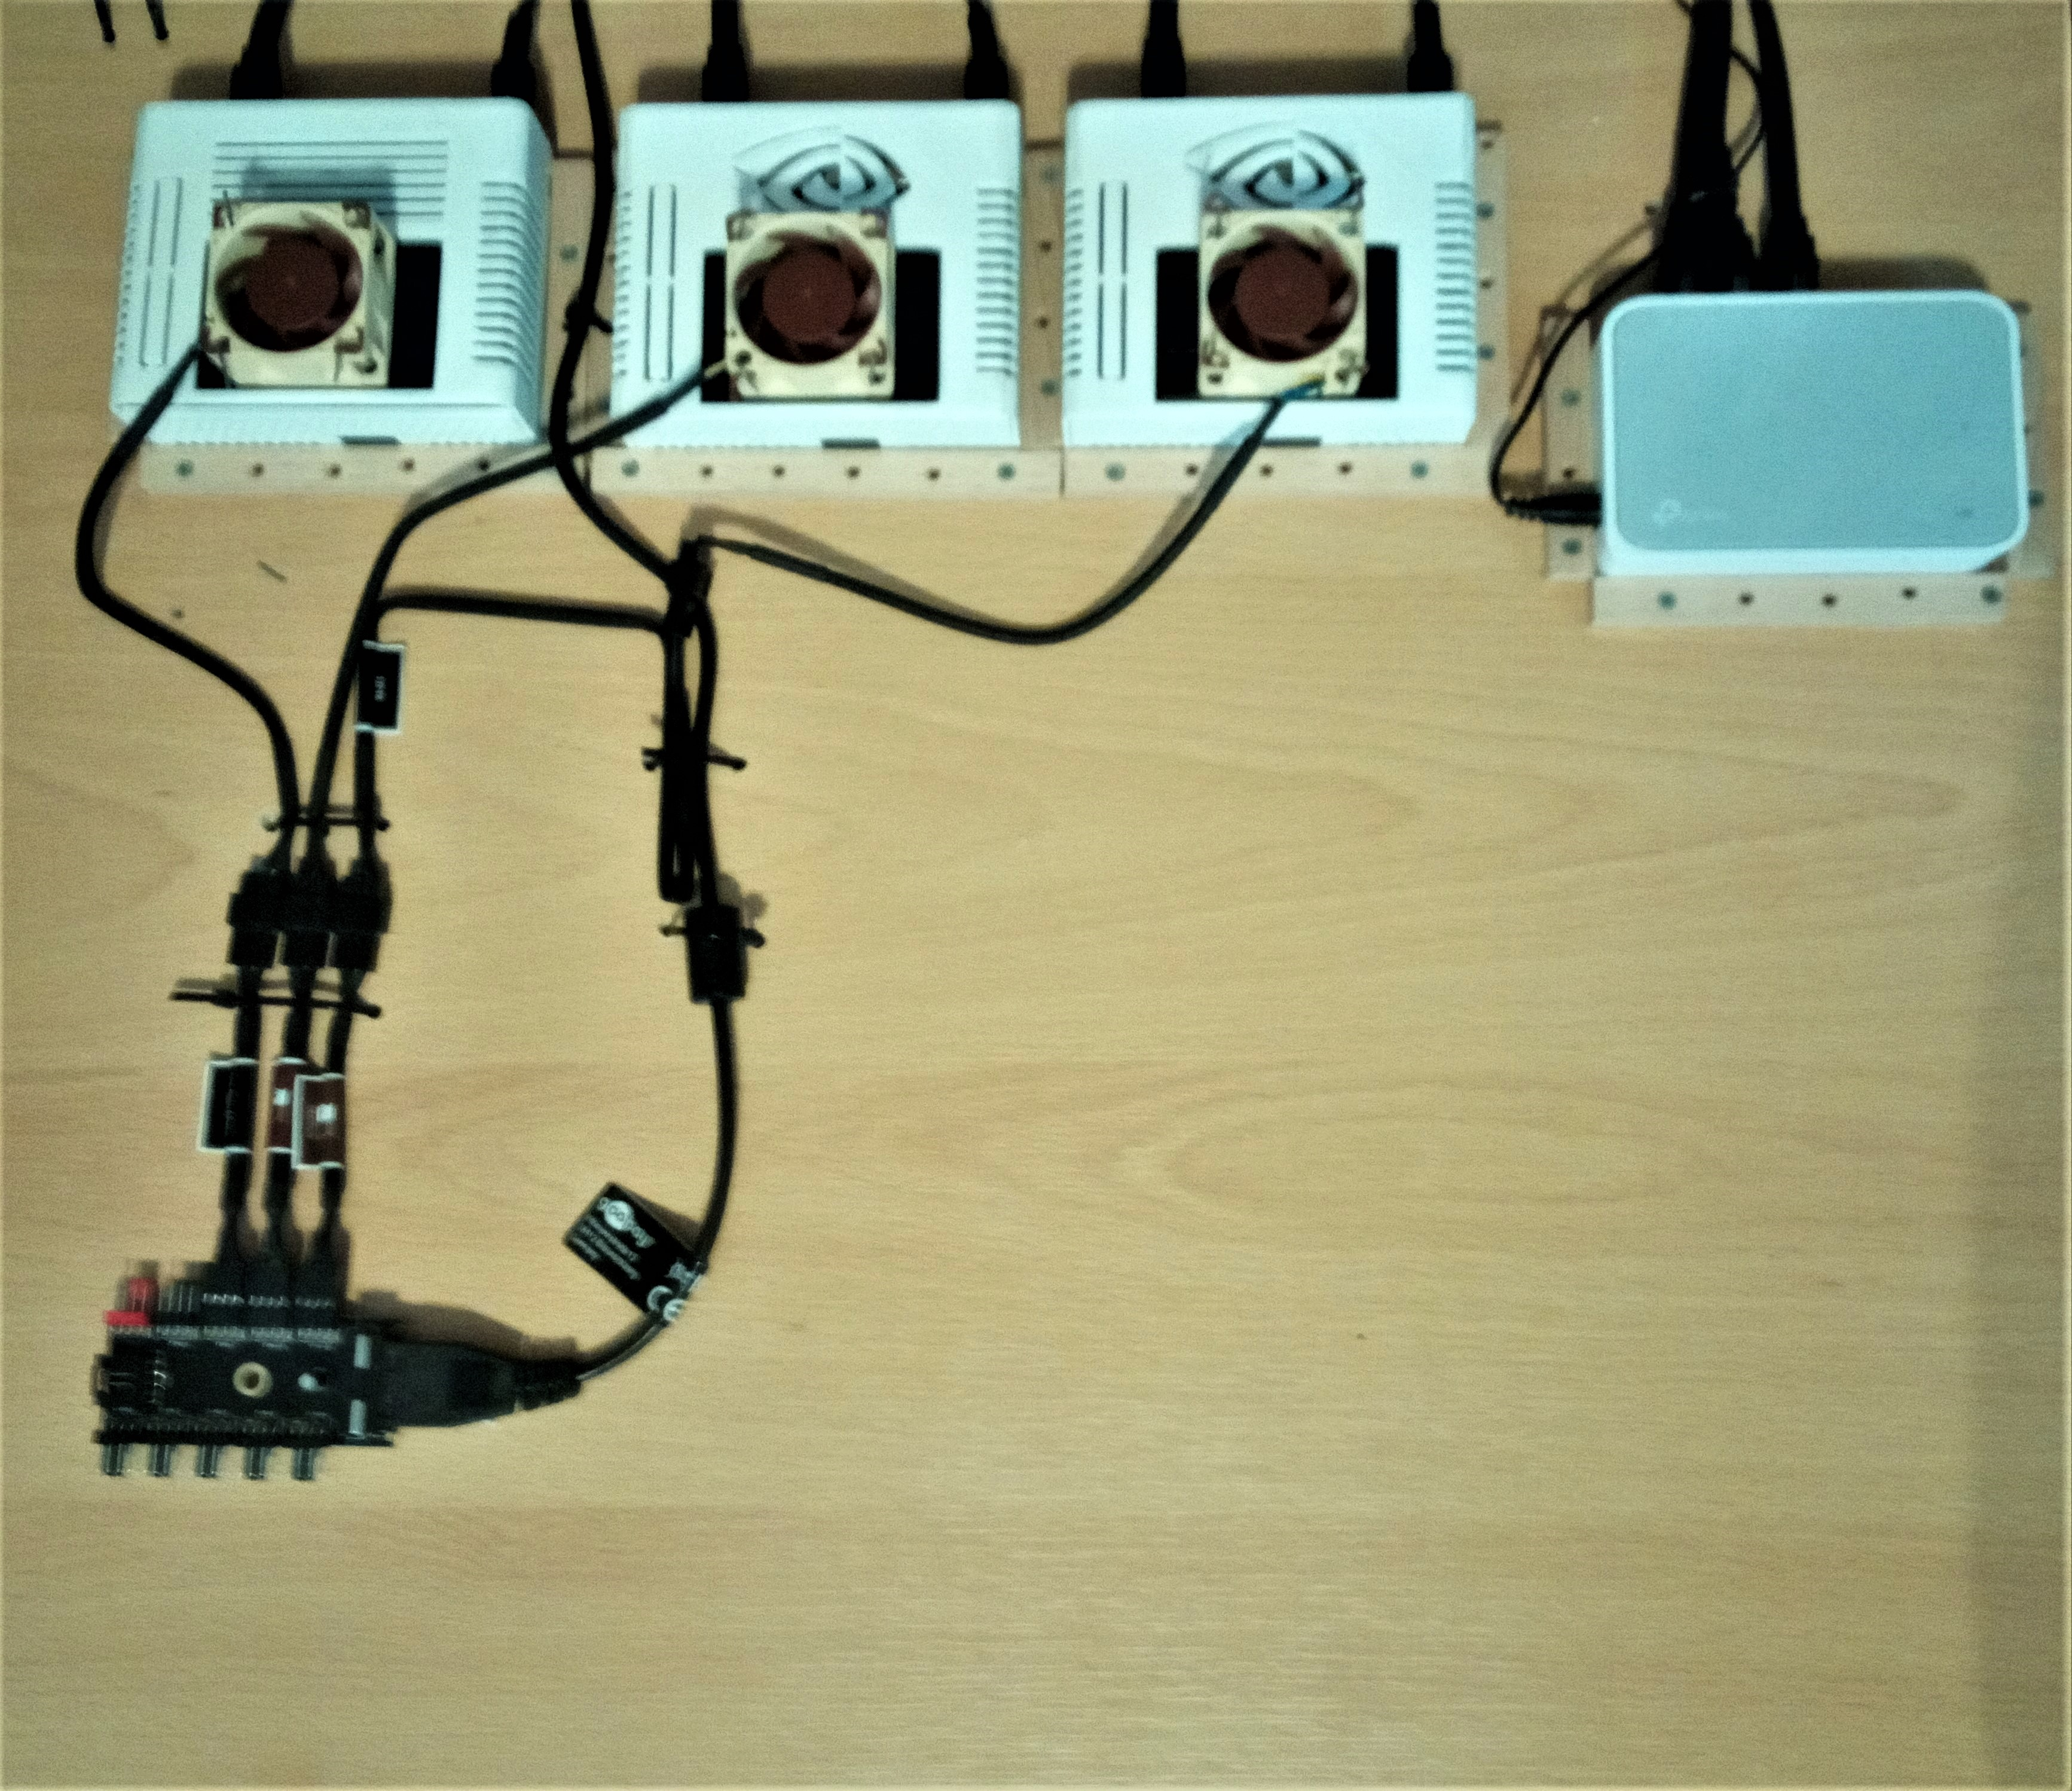
\includegraphics[width=1.0\textwidth]{images/Foto1.jpg}
	\caption{Der im Rahmen dieses Projektes erstellte Mini-Cluster. Zur besseren Nutzung wurden sowohl die Nvidia Jetson Nanos als auch der Switch durch seitliche Leisten auf einem Holzbrett fixiert. Um die vollständige Leistung durch die Nutzung des Powermodus zu erzielen, wurde desweiteren auf jedem Jetson Nano ein 40mm Lüfter installiert. Für die Steuerung dieser Lüfter wurde ein externer Lüfter-Controller genutzt, weil die Lüfter eine Betriebsspannung von 12V benötigen, der Jetson Nano jedoch nur Lüfter mit 5V Betriebsspannung unterstützt.}
	\label{img:foto1}
\end{figure}
\end{appendix}
\newpage
\bibliography{literatur}{}
\addcontentsline{toc}{section}{Literatur}  
\end{document}
